\documentclass[]{article}
\usepackage{lmodern}
\usepackage{amssymb,amsmath}
\usepackage{ifxetex,ifluatex}
\usepackage{fixltx2e} % provides \textsubscript
\ifnum 0\ifxetex 1\fi\ifluatex 1\fi=0 % if pdftex
  \usepackage[T1]{fontenc}
  \usepackage[utf8]{inputenc}
\else % if luatex or xelatex
  \ifxetex
    \usepackage{mathspec}
  \else
    \usepackage{fontspec}
  \fi
  \defaultfontfeatures{Ligatures=TeX,Scale=MatchLowercase}
\fi
% use upquote if available, for straight quotes in verbatim environments
\IfFileExists{upquote.sty}{\usepackage{upquote}}{}
% use microtype if available
\IfFileExists{microtype.sty}{%
\usepackage{microtype}
\UseMicrotypeSet[protrusion]{basicmath} % disable protrusion for tt fonts
}{}
\usepackage[margin=1in]{geometry}
\usepackage{hyperref}
\hypersetup{unicode=true,
            pdftitle={Summary Graphs of NUTR630 Post-Semester Feedback},
            pdfauthor={Dave Bridges, Liv Anderson and Rina Hisamatsu},
            pdfborder={0 0 0},
            breaklinks=true}
\urlstyle{same}  % don't use monospace font for urls
\usepackage{color}
\usepackage{fancyvrb}
\newcommand{\VerbBar}{|}
\newcommand{\VERB}{\Verb[commandchars=\\\{\}]}
\DefineVerbatimEnvironment{Highlighting}{Verbatim}{commandchars=\\\{\}}
% Add ',fontsize=\small' for more characters per line
\usepackage{framed}
\definecolor{shadecolor}{RGB}{248,248,248}
\newenvironment{Shaded}{\begin{snugshade}}{\end{snugshade}}
\newcommand{\KeywordTok}[1]{\textcolor[rgb]{0.13,0.29,0.53}{\textbf{{#1}}}}
\newcommand{\DataTypeTok}[1]{\textcolor[rgb]{0.13,0.29,0.53}{{#1}}}
\newcommand{\DecValTok}[1]{\textcolor[rgb]{0.00,0.00,0.81}{{#1}}}
\newcommand{\BaseNTok}[1]{\textcolor[rgb]{0.00,0.00,0.81}{{#1}}}
\newcommand{\FloatTok}[1]{\textcolor[rgb]{0.00,0.00,0.81}{{#1}}}
\newcommand{\ConstantTok}[1]{\textcolor[rgb]{0.00,0.00,0.00}{{#1}}}
\newcommand{\CharTok}[1]{\textcolor[rgb]{0.31,0.60,0.02}{{#1}}}
\newcommand{\SpecialCharTok}[1]{\textcolor[rgb]{0.00,0.00,0.00}{{#1}}}
\newcommand{\StringTok}[1]{\textcolor[rgb]{0.31,0.60,0.02}{{#1}}}
\newcommand{\VerbatimStringTok}[1]{\textcolor[rgb]{0.31,0.60,0.02}{{#1}}}
\newcommand{\SpecialStringTok}[1]{\textcolor[rgb]{0.31,0.60,0.02}{{#1}}}
\newcommand{\ImportTok}[1]{{#1}}
\newcommand{\CommentTok}[1]{\textcolor[rgb]{0.56,0.35,0.01}{\textit{{#1}}}}
\newcommand{\DocumentationTok}[1]{\textcolor[rgb]{0.56,0.35,0.01}{\textbf{\textit{{#1}}}}}
\newcommand{\AnnotationTok}[1]{\textcolor[rgb]{0.56,0.35,0.01}{\textbf{\textit{{#1}}}}}
\newcommand{\CommentVarTok}[1]{\textcolor[rgb]{0.56,0.35,0.01}{\textbf{\textit{{#1}}}}}
\newcommand{\OtherTok}[1]{\textcolor[rgb]{0.56,0.35,0.01}{{#1}}}
\newcommand{\FunctionTok}[1]{\textcolor[rgb]{0.00,0.00,0.00}{{#1}}}
\newcommand{\VariableTok}[1]{\textcolor[rgb]{0.00,0.00,0.00}{{#1}}}
\newcommand{\ControlFlowTok}[1]{\textcolor[rgb]{0.13,0.29,0.53}{\textbf{{#1}}}}
\newcommand{\OperatorTok}[1]{\textcolor[rgb]{0.81,0.36,0.00}{\textbf{{#1}}}}
\newcommand{\BuiltInTok}[1]{{#1}}
\newcommand{\ExtensionTok}[1]{{#1}}
\newcommand{\PreprocessorTok}[1]{\textcolor[rgb]{0.56,0.35,0.01}{\textit{{#1}}}}
\newcommand{\AttributeTok}[1]{\textcolor[rgb]{0.77,0.63,0.00}{{#1}}}
\newcommand{\RegionMarkerTok}[1]{{#1}}
\newcommand{\InformationTok}[1]{\textcolor[rgb]{0.56,0.35,0.01}{\textbf{\textit{{#1}}}}}
\newcommand{\WarningTok}[1]{\textcolor[rgb]{0.56,0.35,0.01}{\textbf{\textit{{#1}}}}}
\newcommand{\AlertTok}[1]{\textcolor[rgb]{0.94,0.16,0.16}{{#1}}}
\newcommand{\ErrorTok}[1]{\textcolor[rgb]{0.64,0.00,0.00}{\textbf{{#1}}}}
\newcommand{\NormalTok}[1]{{#1}}
\usepackage{graphicx,grffile}
\makeatletter
\def\maxwidth{\ifdim\Gin@nat@width>\linewidth\linewidth\else\Gin@nat@width\fi}
\def\maxheight{\ifdim\Gin@nat@height>\textheight\textheight\else\Gin@nat@height\fi}
\makeatother
% Scale images if necessary, so that they will not overflow the page
% margins by default, and it is still possible to overwrite the defaults
% using explicit options in \includegraphics[width, height, ...]{}
\setkeys{Gin}{width=\maxwidth,height=\maxheight,keepaspectratio}
\IfFileExists{parskip.sty}{%
\usepackage{parskip}
}{% else
\setlength{\parindent}{0pt}
\setlength{\parskip}{6pt plus 2pt minus 1pt}
}
\setlength{\emergencystretch}{3em}  % prevent overfull lines
\providecommand{\tightlist}{%
  \setlength{\itemsep}{0pt}\setlength{\parskip}{0pt}}
\setcounter{secnumdepth}{0}
% Redefines (sub)paragraphs to behave more like sections
\ifx\paragraph\undefined\else
\let\oldparagraph\paragraph
\renewcommand{\paragraph}[1]{\oldparagraph{#1}\mbox{}}
\fi
\ifx\subparagraph\undefined\else
\let\oldsubparagraph\subparagraph
\renewcommand{\subparagraph}[1]{\oldsubparagraph{#1}\mbox{}}
\fi

%%% Use protect on footnotes to avoid problems with footnotes in titles
\let\rmarkdownfootnote\footnote%
\def\footnote{\protect\rmarkdownfootnote}

%%% Change title format to be more compact
\usepackage{titling}

% Create subtitle command for use in maketitle
\newcommand{\subtitle}[1]{
  \posttitle{
    \begin{center}\large#1\end{center}
    }
}

\setlength{\droptitle}{-2em}
  \title{Summary Graphs of NUTR630 Post-Semester Feedback}
  \pretitle{\vspace{\droptitle}\centering\huge}
  \posttitle{\par}
  \author{Dave Bridges, Liv Anderson and Rina Hisamatsu}
  \preauthor{\centering\large\emph}
  \postauthor{\par}
  \predate{\centering\large\emph}
  \postdate{\par}
  \date{2017-09-03}


\begin{document}
\maketitle

{
\setcounter{tocdepth}{2}
\tableofcontents
}
\begin{Shaded}
\begin{Highlighting}[]
\KeywordTok{library}\NormalTok{(readr)}
\NormalTok{onboarding.filename <-}\StringTok{ 'https://docs.google.com/spreadsheets/d/e/2PACX-1vQI-b1A4Zd-gx3FuY3lkKbWE0zKUfmAhpFovKOxow5AC1wWQpBsSvOKI0_gtZ4DJu5sj-YM1_1nsKUe/pub?gid=1032535237&single=true&output=csv'}
\NormalTok{onboarding.data <-}\StringTok{ }\KeywordTok{read_csv}\NormalTok{(onboarding.filename)}

\NormalTok{end.filename <-}\StringTok{ 'https://docs.google.com/spreadsheets/d/e/2PACX-1vTxPKhKOwkZ18U1X0Z44M8wGqtM5ow18tVPF4yupZbzditOQdlQ3DJkfJJA-Dl226NfGYJ0tEUqOFn4/pub?gid=1563141647&single=true&output=csv'}
\NormalTok{end.data <-}\StringTok{ }\KeywordTok{read_csv}\NormalTok{(end.filename)}

\NormalTok{merged.data <-}\StringTok{ }\KeywordTok{full_join}\NormalTok{(onboarding.data,end.data, }\DataTypeTok{by=}\StringTok{'Email Address'}\NormalTok{, }\DataTypeTok{suffix=}\KeywordTok{c}\NormalTok{(}\StringTok{"before"}\NormalTok{,}\StringTok{"after"}\NormalTok{))}
\end{Highlighting}
\end{Shaded}

These data can be found in
/Users/davebrid/Documents/GitHub/TeachingLectures/Michigan/NUTR630/Evaluation/GradeCraft
Summary/Student Feedback/Post-Semester. This script was most recently
updated on Wed Jan 31 17:41:34 2018.

\section{Analysis}\label{analysis}

\subsection{Interests}\label{interests}

\subsection{Learning Activities}\label{learning-activities}

\subsubsection{Thoughts about whether they learned a lot from the
activity}\label{thoughts-about-whether-they-learned-a-lot-from-the-activity}

\begin{Shaded}
\begin{Highlighting}[]
\KeywordTok{library}\NormalTok{(dplyr)}

\NormalTok{mylevels <-}\StringTok{ }\KeywordTok{c}\NormalTok{(}\StringTok{'Strongly Agree'}\NormalTok{,}\StringTok{'Agree'}\NormalTok{,}\StringTok{'Neutral'}\NormalTok{,}\StringTok{'Disagree'}\NormalTok{,}\StringTok{'Strongly Disagree'}\NormalTok{)}


\NormalTok{activity.data <-}\StringTok{ }
\StringTok{  }\NormalTok{end.data %>%}
\StringTok{  }\NormalTok{dplyr::}\KeywordTok{select}\NormalTok{(}\KeywordTok{contains}\NormalTok{(}\StringTok{"learned"}\NormalTok{)) %>%}
\StringTok{  }\KeywordTok{rename}\NormalTok{(}\StringTok{`}\DataTypeTok{Written Reports}\StringTok{`} \NormalTok{=}\StringTok{ `}\DataTypeTok{Select one in reference to written reports [I learned a lot from this activity]}\StringTok{`}\NormalTok{,}
         \StringTok{`}\DataTypeTok{Presentation}\StringTok{`} \NormalTok{=}\StringTok{ `}\DataTypeTok{Select one in reference to your presentation [I learned a lot from this activity]}\StringTok{`}\NormalTok{,}
         \StringTok{`}\DataTypeTok{Peer Reviews}\StringTok{`} \NormalTok{=}\StringTok{ `}\DataTypeTok{Select one answer in reference to the peer reviews [I learned a lot from this activity]}\StringTok{`}\NormalTok{,}
         \StringTok{`}\DataTypeTok{Social Media}\StringTok{`} \NormalTok{=}\StringTok{ `}\DataTypeTok{Select one in reference to the social media assignments [I learned a lot from this activity]}\StringTok{`}\NormalTok{,}
         \StringTok{`}\DataTypeTok{News Posts}\StringTok{`} \NormalTok{=}\StringTok{ `}\DataTypeTok{Select one in reference to the news posts [I learned a lot from this activity]}\StringTok{`}\NormalTok{,}
         \StringTok{`}\DataTypeTok{Review Questions}\StringTok{`} \NormalTok{=}\StringTok{ `}\DataTypeTok{Select one in reference to the review questions [I learned a lot from this activity]}\StringTok{`}\NormalTok{,}
         \StringTok{`}\DataTypeTok{Problem Roulette}\StringTok{`} \NormalTok{=}\StringTok{ `}\DataTypeTok{Select one answer in reference to problem roulette [I learned a lot from this activity]}\StringTok{`}\NormalTok{) %>%}
\StringTok{  }\KeywordTok{mutate}\NormalTok{(}\StringTok{`}\DataTypeTok{Written Reports}\StringTok{`} \NormalTok{=}\StringTok{ }\KeywordTok{factor}\NormalTok{(}\StringTok{`}\DataTypeTok{Written Reports}\StringTok{`}\NormalTok{,}\DataTypeTok{levels=}\NormalTok{mylevels),}
         \StringTok{`}\DataTypeTok{Presentation}\StringTok{`}\NormalTok{=}\StringTok{ }\KeywordTok{factor}\NormalTok{(}\StringTok{`}\DataTypeTok{Presentation}\StringTok{`}\NormalTok{, }\DataTypeTok{levels=}\NormalTok{mylevels),}
         \StringTok{`}\DataTypeTok{Peer Reviews}\StringTok{`}\NormalTok{=}\StringTok{ }\KeywordTok{factor}\NormalTok{(}\StringTok{`}\DataTypeTok{Peer Reviews}\StringTok{`}\NormalTok{, }\DataTypeTok{levels=}\NormalTok{mylevels),}
         \StringTok{`}\DataTypeTok{Social Media}\StringTok{`}\NormalTok{=}\StringTok{ }\KeywordTok{factor}\NormalTok{(}\StringTok{`}\DataTypeTok{Social Media}\StringTok{`}\NormalTok{, }\DataTypeTok{levels=}\NormalTok{mylevels),}
         \StringTok{`}\DataTypeTok{News Posts}\StringTok{`}\NormalTok{=}\StringTok{ }\KeywordTok{factor}\NormalTok{(}\StringTok{`}\DataTypeTok{News Posts}\StringTok{`}\NormalTok{, }\DataTypeTok{levels=}\NormalTok{mylevels),}
         \StringTok{`}\DataTypeTok{Review Questions}\StringTok{`}\NormalTok{=}\StringTok{ }\KeywordTok{factor}\NormalTok{(}\StringTok{`}\DataTypeTok{Review Questions}\StringTok{`}\NormalTok{, }\DataTypeTok{levels=}\NormalTok{mylevels),}
         \StringTok{`}\DataTypeTok{Problem Roulette}\StringTok{`}\NormalTok{=}\StringTok{ }\KeywordTok{factor}\NormalTok{(}\StringTok{`}\DataTypeTok{Problem Roulette}\StringTok{`}\NormalTok{, }\DataTypeTok{levels=}\NormalTok{mylevels))}

\KeywordTok{library}\NormalTok{(sjPlot)}
\KeywordTok{sjp.likert}\NormalTok{(activity.data, }\DataTypeTok{title=}\StringTok{"I learned a lot from this activity"}\NormalTok{)}
\end{Highlighting}
\end{Shaded}

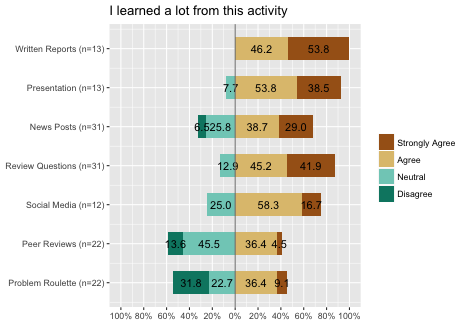
\includegraphics{figures/learning-activities-1.png}

\subsubsection{Thoughts about whether these assesed
knowledge}\label{thoughts-about-whether-these-assesed-knowledge}

\begin{Shaded}
\begin{Highlighting}[]
\NormalTok{assessed.data <-}\StringTok{ }
\StringTok{  }\NormalTok{end.data %>%}
\StringTok{  }\NormalTok{dplyr::}\KeywordTok{select}\NormalTok{(}\KeywordTok{contains}\NormalTok{(}\StringTok{"assessed"}\NormalTok{)) %>%}
\StringTok{  }\KeywordTok{rename}\NormalTok{(}\StringTok{`}\DataTypeTok{Written Reports}\StringTok{`} \NormalTok{=}\StringTok{ `}\DataTypeTok{Select one in reference to written reports [This effectively assessed my knowledge]}\StringTok{`}\NormalTok{,}
         \StringTok{`}\DataTypeTok{Presentation}\StringTok{`} \NormalTok{=}\StringTok{ `}\DataTypeTok{Select one in reference to your presentation [This effectively assessed my knowledge]}\StringTok{`}\NormalTok{,}
         \StringTok{`}\DataTypeTok{Peer Reviews}\StringTok{`} \NormalTok{=}\StringTok{ `}\DataTypeTok{Select one answer in reference to the peer reviews [This effectively assessed my knowledge]}\StringTok{`}\NormalTok{,}
         \StringTok{`}\DataTypeTok{Social Media}\StringTok{`} \NormalTok{=}\StringTok{ `}\DataTypeTok{Select one in reference to the social media assignments [This effectively assessed my knowledge]}\StringTok{`}\NormalTok{,}
         \StringTok{`}\DataTypeTok{News Posts}\StringTok{`} \NormalTok{=}\StringTok{ `}\DataTypeTok{Select one in reference to the news posts [This effectively assessed my knowledge]}\StringTok{`}\NormalTok{,}
         \StringTok{`}\DataTypeTok{Review Questions}\StringTok{`} \NormalTok{=}\StringTok{ `}\DataTypeTok{Select one in reference to the review questions [This effectively assessed my knowledge]}\StringTok{`}\NormalTok{,}
         \StringTok{`}\DataTypeTok{Problem Roulette}\StringTok{`} \NormalTok{=}\StringTok{ `}\DataTypeTok{Select one answer in reference to problem roulette [This effectively assessed my knowledge]}\StringTok{`}\NormalTok{) %>%}
\StringTok{  }\KeywordTok{mutate}\NormalTok{(}\StringTok{`}\DataTypeTok{Written Reports}\StringTok{`} \NormalTok{=}\StringTok{ }\KeywordTok{factor}\NormalTok{(}\StringTok{`}\DataTypeTok{Written Reports}\StringTok{`}\NormalTok{,}\DataTypeTok{levels=}\NormalTok{mylevels),}
         \StringTok{`}\DataTypeTok{Presentation}\StringTok{`}\NormalTok{=}\StringTok{ }\KeywordTok{factor}\NormalTok{(}\StringTok{`}\DataTypeTok{Presentation}\StringTok{`}\NormalTok{, }\DataTypeTok{levels=}\NormalTok{mylevels),}
         \StringTok{`}\DataTypeTok{Peer Reviews}\StringTok{`}\NormalTok{=}\StringTok{ }\KeywordTok{factor}\NormalTok{(}\StringTok{`}\DataTypeTok{Peer Reviews}\StringTok{`}\NormalTok{, }\DataTypeTok{levels=}\NormalTok{mylevels),}
         \StringTok{`}\DataTypeTok{Social Media}\StringTok{`}\NormalTok{=}\StringTok{ }\KeywordTok{factor}\NormalTok{(}\StringTok{`}\DataTypeTok{Social Media}\StringTok{`}\NormalTok{, }\DataTypeTok{levels=}\NormalTok{mylevels),}
         \StringTok{`}\DataTypeTok{News Posts}\StringTok{`}\NormalTok{=}\StringTok{ }\KeywordTok{factor}\NormalTok{(}\StringTok{`}\DataTypeTok{News Posts}\StringTok{`}\NormalTok{, }\DataTypeTok{levels=}\NormalTok{mylevels),}
         \StringTok{`}\DataTypeTok{Review Questions}\StringTok{`}\NormalTok{=}\StringTok{ }\KeywordTok{factor}\NormalTok{(}\StringTok{`}\DataTypeTok{Review Questions}\StringTok{`}\NormalTok{, }\DataTypeTok{levels=}\NormalTok{mylevels),}
         \StringTok{`}\DataTypeTok{Problem Roulette}\StringTok{`}\NormalTok{=}\StringTok{ }\KeywordTok{factor}\NormalTok{(}\StringTok{`}\DataTypeTok{Problem Roulette}\StringTok{`}\NormalTok{, }\DataTypeTok{levels=}\NormalTok{mylevels))}

\KeywordTok{sjp.likert}\NormalTok{(assessed.data, }\DataTypeTok{title=}\StringTok{"This effectively assessed my knowledge"}\NormalTok{)}
\end{Highlighting}
\end{Shaded}

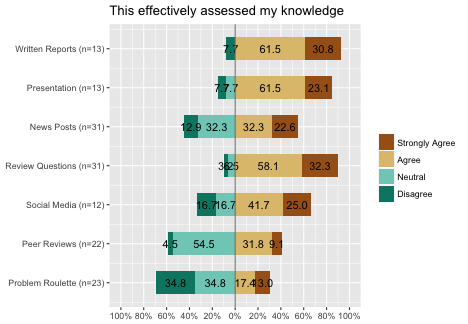
\includegraphics{figures/assessed-knowledge-1.png}

\subsubsection{Thoughts as to whether it was worth an ppropriate amount
of
points}\label{thoughts-as-to-whether-it-was-worth-an-ppropriate-amount-of-points}

\begin{Shaded}
\begin{Highlighting}[]
\NormalTok{points.data <-}\StringTok{ }
\StringTok{  }\NormalTok{end.data %>%}
\StringTok{  }\NormalTok{dplyr::}\KeywordTok{select}\NormalTok{(}\KeywordTok{contains}\NormalTok{(}\StringTok{"appropriate amount"}\NormalTok{)) %>%}
\StringTok{  }\KeywordTok{rename}\NormalTok{(}\StringTok{`}\DataTypeTok{Written Reports}\StringTok{`} \NormalTok{=}\StringTok{ `}\DataTypeTok{Select one in reference to written reports [This was worth an appropriate amount of points based on the amount of effort required]}\StringTok{`}\NormalTok{,}
         \StringTok{`}\DataTypeTok{Presentation}\StringTok{`} \NormalTok{=}\StringTok{ `}\DataTypeTok{Select one in reference to your presentation [This was worth an appropriate amount of points based on the amount of effort required]}\StringTok{`}\NormalTok{,}
         \StringTok{`}\DataTypeTok{Peer Reviews}\StringTok{`} \NormalTok{=}\StringTok{ `}\DataTypeTok{Select one answer in reference to the peer reviews [This was worth an appropriate amount of points based on the amount of effort required]}\StringTok{`}\NormalTok{,}
         \StringTok{`}\DataTypeTok{Social Media}\StringTok{`} \NormalTok{=}\StringTok{ `}\DataTypeTok{Select one in reference to the social media assignments [This was worth an appropriate amount of points based on the amount of effort required]}\StringTok{`}\NormalTok{,}
         \StringTok{`}\DataTypeTok{News Posts}\StringTok{`} \NormalTok{=}\StringTok{ `}\DataTypeTok{Select one in reference to the news posts [This was worth an appropriate amount of points based on the amount of effort required]}\StringTok{`}\NormalTok{,}
         \StringTok{`}\DataTypeTok{Review Questions}\StringTok{`} \NormalTok{=}\StringTok{ `}\DataTypeTok{Select one in reference to the review questions [This was worth an appropriate amount of points based on the amount of effort required]}\StringTok{`}\NormalTok{,}
         \StringTok{`}\DataTypeTok{Problem Roulette}\StringTok{`} \NormalTok{=}\StringTok{ `}\DataTypeTok{Select one answer in reference to problem roulette [This was worth an appropriate amount of points based on the amount of effort required]}\StringTok{`}\NormalTok{) %>%}
\StringTok{  }\KeywordTok{mutate}\NormalTok{(}\StringTok{`}\DataTypeTok{Written Reports}\StringTok{`} \NormalTok{=}\StringTok{ }\KeywordTok{factor}\NormalTok{(}\StringTok{`}\DataTypeTok{Written Reports}\StringTok{`}\NormalTok{,}\DataTypeTok{levels=}\NormalTok{mylevels),}
         \StringTok{`}\DataTypeTok{Presentation}\StringTok{`}\NormalTok{=}\StringTok{ }\KeywordTok{factor}\NormalTok{(}\StringTok{`}\DataTypeTok{Presentation}\StringTok{`}\NormalTok{, }\DataTypeTok{levels=}\NormalTok{mylevels),}
         \StringTok{`}\DataTypeTok{Peer Reviews}\StringTok{`}\NormalTok{=}\StringTok{ }\KeywordTok{factor}\NormalTok{(}\StringTok{`}\DataTypeTok{Peer Reviews}\StringTok{`}\NormalTok{, }\DataTypeTok{levels=}\NormalTok{mylevels),}
         \StringTok{`}\DataTypeTok{Social Media}\StringTok{`}\NormalTok{=}\StringTok{ }\KeywordTok{factor}\NormalTok{(}\StringTok{`}\DataTypeTok{Social Media}\StringTok{`}\NormalTok{, }\DataTypeTok{levels=}\NormalTok{mylevels),}
         \StringTok{`}\DataTypeTok{News Posts}\StringTok{`}\NormalTok{=}\StringTok{ }\KeywordTok{factor}\NormalTok{(}\StringTok{`}\DataTypeTok{News Posts}\StringTok{`}\NormalTok{, }\DataTypeTok{levels=}\NormalTok{mylevels),}
         \StringTok{`}\DataTypeTok{Review Questions}\StringTok{`}\NormalTok{=}\StringTok{ }\KeywordTok{factor}\NormalTok{(}\StringTok{`}\DataTypeTok{Review Questions}\StringTok{`}\NormalTok{, }\DataTypeTok{levels=}\NormalTok{mylevels),}
         \StringTok{`}\DataTypeTok{Problem Roulette}\StringTok{`}\NormalTok{=}\StringTok{ }\KeywordTok{factor}\NormalTok{(}\StringTok{`}\DataTypeTok{Problem Roulette}\StringTok{`}\NormalTok{, }\DataTypeTok{levels=}\NormalTok{mylevels))}

\KeywordTok{sjp.likert}\NormalTok{(points.data, }\DataTypeTok{title=}\StringTok{"This was worth an appropriate amount of points based on the amount of effort required"}\NormalTok{)}
\end{Highlighting}
\end{Shaded}

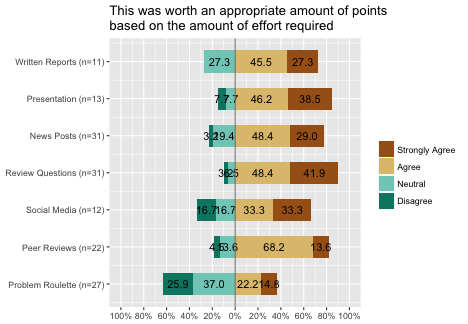
\includegraphics{figures/amount-of-points-1.png}

\section{Changes over the semester}\label{changes-over-the-semester}

\subsection{Interests and Aptitudes}\label{interests-and-aptitudes}

\begin{Shaded}
\begin{Highlighting}[]
\NormalTok{merged.data[merged.data==}\DecValTok{1}\NormalTok{]<-}\StringTok{'Strongly Agree'}
\NormalTok{merged.data[merged.data==}\DecValTok{2}\NormalTok{]<-}\StringTok{'Agree'}
\NormalTok{merged.data[merged.data==}\DecValTok{3}\NormalTok{]<-}\StringTok{'Neutral'}
\NormalTok{merged.data[merged.data==}\DecValTok{4}\NormalTok{]<-}\StringTok{'Disagree'}
\NormalTok{merged.data[merged.data==}\DecValTok{5}\NormalTok{]<-}\StringTok{'Strongly Disagree'}


\NormalTok{macronutritent.aptitude.data <-}\StringTok{ }
\StringTok{  }\NormalTok{merged.data %>%}
\StringTok{  }\NormalTok{dplyr::}\KeywordTok{select}\NormalTok{(}\KeywordTok{contains}\NormalTok{(}\StringTok{"macronutrient"}\NormalTok{)) %>%}
\StringTok{  }\KeywordTok{rename}\NormalTok{(}\StringTok{`}\DataTypeTok{Interested Before}\StringTok{`} \NormalTok{=}\StringTok{ `}\DataTypeTok{Macronutrient biochemistry is of interest to me.before}\StringTok{`}\NormalTok{,}
         \StringTok{`}\DataTypeTok{Interested After}\StringTok{`} \NormalTok{=}\StringTok{ `}\DataTypeTok{Macronutrient biochemistry is of interest to me.after}\StringTok{`}\NormalTok{,}
         \StringTok{`}\DataTypeTok{Important Before}\StringTok{`} \NormalTok{=}\StringTok{ `}\DataTypeTok{Macronutrient biochemistry is important for my career interests.before}\StringTok{`}\NormalTok{,}
         \StringTok{`}\DataTypeTok{Important After}\StringTok{`} \NormalTok{=}\StringTok{ `}\DataTypeTok{Macronutrient biochemistry is important for my career interests.after}\StringTok{`}\NormalTok{) %>%}
\StringTok{  }\KeywordTok{mutate}\NormalTok{(}\StringTok{`}\DataTypeTok{Interested Before}\StringTok{`}\NormalTok{=}\StringTok{ }\KeywordTok{factor}\NormalTok{(}\StringTok{`}\DataTypeTok{Interested Before}\StringTok{`}\NormalTok{, }\DataTypeTok{levels=}\NormalTok{mylevels),}
         \StringTok{`}\DataTypeTok{Interested After}\StringTok{`}\NormalTok{=}\StringTok{ }\KeywordTok{factor}\NormalTok{(}\StringTok{`}\DataTypeTok{Interested After}\StringTok{`}\NormalTok{, }\DataTypeTok{levels=}\NormalTok{mylevels),}
         \StringTok{`}\DataTypeTok{Important Before}\StringTok{`}\NormalTok{=}\StringTok{ }\KeywordTok{factor}\NormalTok{(}\StringTok{`}\DataTypeTok{Important Before}\StringTok{`}\NormalTok{, }\DataTypeTok{levels=}\NormalTok{mylevels),}
         \StringTok{`}\DataTypeTok{Important After}\StringTok{`}\NormalTok{=}\StringTok{ }\KeywordTok{factor}\NormalTok{(}\StringTok{`}\DataTypeTok{Important After}\StringTok{`}\NormalTok{, }\DataTypeTok{levels=}\NormalTok{mylevels))}
\NormalTok{col.order <-}\StringTok{ }\KeywordTok{c}\NormalTok{(}\DecValTok{1}\NormalTok{,}\DecValTok{3}\NormalTok{,}\DecValTok{2}\NormalTok{,}\DecValTok{4}\NormalTok{)}

\KeywordTok{sjp.likert}\NormalTok{(macronutritent.aptitude.data[,col.order], }\DataTypeTok{title=}\StringTok{"Macronutrient biochemistry"}\NormalTok{)}
\end{Highlighting}
\end{Shaded}

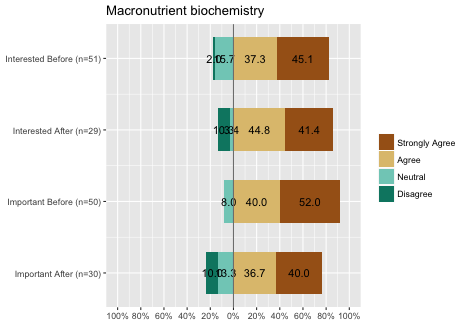
\includegraphics{figures/interests-1.png}

\begin{Shaded}
\begin{Highlighting}[]
\NormalTok{digestive.aptitude.data <-}\StringTok{ }
\StringTok{  }\NormalTok{merged.data %>%}
\StringTok{  }\NormalTok{dplyr::}\KeywordTok{select}\NormalTok{(}\KeywordTok{contains}\NormalTok{(}\StringTok{"digestive"}\NormalTok{)) %>%}
\StringTok{  }\KeywordTok{rename}\NormalTok{(}\StringTok{`}\DataTypeTok{Interested Before}\StringTok{`} \NormalTok{=}\StringTok{ `}\DataTypeTok{Comprehensive understanding of the digestive tract is of interest to me.before}\StringTok{`}\NormalTok{,}
         \StringTok{`}\DataTypeTok{Interested After}\StringTok{`} \NormalTok{=}\StringTok{ `}\DataTypeTok{Comprehensive understanding of the digestive tract is of interest to me.after}\StringTok{`}\NormalTok{,}
         \StringTok{`}\DataTypeTok{Important Before}\StringTok{`} \NormalTok{=}\StringTok{ `}\DataTypeTok{Comprehensive understanding of the digestive tract is important for my career interests.before}\StringTok{`}\NormalTok{,}
         \StringTok{`}\DataTypeTok{Important After}\StringTok{`} \NormalTok{=}\StringTok{ `}\DataTypeTok{Comprehensive understanding of the digestive tract is important for my career interests.after}\StringTok{`}\NormalTok{) %>%}
\StringTok{  }\KeywordTok{mutate}\NormalTok{(}\StringTok{`}\DataTypeTok{Interested Before}\StringTok{`}\NormalTok{=}\StringTok{ }\KeywordTok{factor}\NormalTok{(}\StringTok{`}\DataTypeTok{Interested Before}\StringTok{`}\NormalTok{, }\DataTypeTok{levels=}\NormalTok{mylevels),}
         \StringTok{`}\DataTypeTok{Interested After}\StringTok{`}\NormalTok{=}\StringTok{ }\KeywordTok{factor}\NormalTok{(}\StringTok{`}\DataTypeTok{Interested After}\StringTok{`}\NormalTok{, }\DataTypeTok{levels=}\NormalTok{mylevels),}
         \StringTok{`}\DataTypeTok{Important Before}\StringTok{`}\NormalTok{=}\StringTok{ }\KeywordTok{factor}\NormalTok{(}\StringTok{`}\DataTypeTok{Important Before}\StringTok{`}\NormalTok{, }\DataTypeTok{levels=}\NormalTok{mylevels),}
         \StringTok{`}\DataTypeTok{Important After}\StringTok{`}\NormalTok{=}\StringTok{ }\KeywordTok{factor}\NormalTok{(}\StringTok{`}\DataTypeTok{Important After}\StringTok{`}\NormalTok{, }\DataTypeTok{levels=}\NormalTok{mylevels))}
\NormalTok{col.order <-}\StringTok{ }\KeywordTok{c}\NormalTok{(}\DecValTok{1}\NormalTok{,}\DecValTok{3}\NormalTok{,}\DecValTok{2}\NormalTok{,}\DecValTok{4}\NormalTok{)}

\KeywordTok{sjp.likert}\NormalTok{(digestive.aptitude.data[,col.order], }\DataTypeTok{title=}\StringTok{"Understanding of the digestive tract"}\NormalTok{)}
\end{Highlighting}
\end{Shaded}

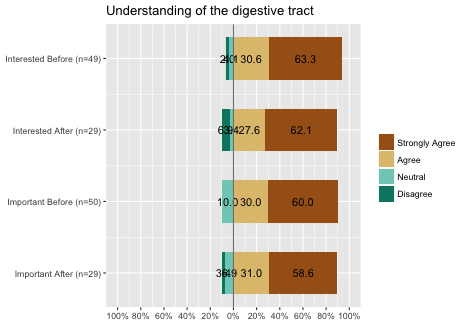
\includegraphics{figures/interests-2.png}

\section{Metacognition}\label{metacognition}

\begin{Shaded}
\begin{Highlighting}[]
\NormalTok{meta.data <-}\StringTok{ }
\StringTok{  }\NormalTok{merged.data %>%}
\StringTok{  }\NormalTok{dplyr::}\KeywordTok{select}\NormalTok{(}\KeywordTok{contains}\NormalTok{(}\StringTok{"What is your level of agreement on the following statements? [When given an assignment to complete, I produce better outcomes with a community of support (i.e., instructor or peer support).]"}\NormalTok{)) %>%}
\StringTok{  }\KeywordTok{rename}\NormalTok{(}\StringTok{`}\DataTypeTok{Before}\StringTok{`} \NormalTok{=}\StringTok{ `}\DataTypeTok{What is your level of agreement on the following statements? [When given an assignment to complete, I produce better outcomes with a community of support (i.e., instructor or peer support).]before}\StringTok{`}\NormalTok{,}
         \StringTok{`}\DataTypeTok{After}\StringTok{`} \NormalTok{=}\StringTok{  `}\DataTypeTok{What is your level of agreement on the following statements? [When given an assignment to complete, I produce better outcomes with a community of support (i.e., instructor or peer support).]after}\StringTok{`}\NormalTok{) %>%}
\StringTok{  }\KeywordTok{mutate}\NormalTok{(}\StringTok{`}\DataTypeTok{Before}\StringTok{`}\NormalTok{=}\StringTok{ }\KeywordTok{factor}\NormalTok{(}\StringTok{`}\DataTypeTok{Before}\StringTok{`}\NormalTok{, }\DataTypeTok{levels=}\NormalTok{mylevels),}
         \StringTok{`}\DataTypeTok{After}\StringTok{`}\NormalTok{=}\StringTok{ }\KeywordTok{factor}\NormalTok{(}\StringTok{`}\DataTypeTok{After}\StringTok{`}\NormalTok{, }\DataTypeTok{levels=}\NormalTok{mylevels))}

\KeywordTok{sjp.likert}\NormalTok{(meta.data, }\DataTypeTok{title=}\StringTok{"When given an assignment to complete, I produce better outcomes with a community of support (i.e., instructor or peer support)"}\NormalTok{, }\DataTypeTok{cat.neutral=}\StringTok{'Neutral'}\NormalTok{)}
\end{Highlighting}
\end{Shaded}

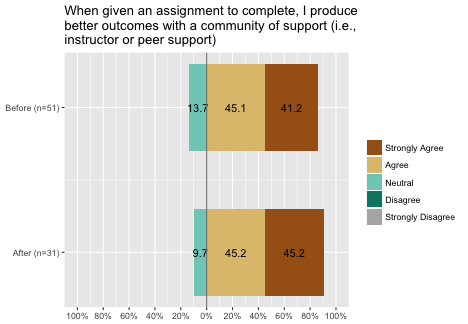
\includegraphics{figures/metacognition-1.png}

\begin{Shaded}
\begin{Highlighting}[]
\NormalTok{meta.data <-}\StringTok{ }
\StringTok{  }\NormalTok{merged.data %>%}
\StringTok{  }\NormalTok{dplyr::}\KeywordTok{select}\NormalTok{(}\KeywordTok{contains}\NormalTok{(}\StringTok{"What is your level of agreement on the following statements? [I am motivated to complete an assignment if I enjoy doing it.]"}\NormalTok{)) %>%}
\StringTok{  }\KeywordTok{rename}\NormalTok{(}\StringTok{`}\DataTypeTok{Before}\StringTok{`} \NormalTok{=}\StringTok{ `}\DataTypeTok{What is your level of agreement on the following statements? [I am motivated to complete an assignment if I enjoy doing it.]before}\StringTok{`}\NormalTok{,}
         \StringTok{`}\DataTypeTok{After}\StringTok{`} \NormalTok{=}\StringTok{  `}\DataTypeTok{What is your level of agreement on the following statements? [I am motivated to complete an assignment if I enjoy doing it.]after}\StringTok{`}\NormalTok{) %>%}
\StringTok{  }\KeywordTok{mutate}\NormalTok{(}\StringTok{`}\DataTypeTok{Before}\StringTok{`}\NormalTok{=}\StringTok{ }\KeywordTok{factor}\NormalTok{(}\StringTok{`}\DataTypeTok{Before}\StringTok{`}\NormalTok{, }\DataTypeTok{levels=}\NormalTok{mylevels),}
         \StringTok{`}\DataTypeTok{After}\StringTok{`}\NormalTok{=}\StringTok{ }\KeywordTok{factor}\NormalTok{(}\StringTok{`}\DataTypeTok{After}\StringTok{`}\NormalTok{, }\DataTypeTok{levels=}\NormalTok{mylevels))}

\KeywordTok{sjp.likert}\NormalTok{(meta.data, }\DataTypeTok{title=}\StringTok{"I am motivated to complete an assignment if I enjoy doing it."}\NormalTok{, }\DataTypeTok{cat.neutral=}\StringTok{'Neutral'}\NormalTok{)}
\end{Highlighting}
\end{Shaded}

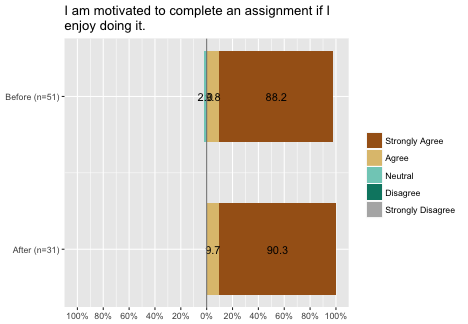
\includegraphics{figures/metacognition-2.png}

\begin{Shaded}
\begin{Highlighting}[]
\NormalTok{meta.data <-}\StringTok{ }
\StringTok{  }\NormalTok{merged.data %>%}
\StringTok{  }\NormalTok{dplyr::}\KeywordTok{select}\NormalTok{(}\KeywordTok{contains}\NormalTok{(}\StringTok{"What is your level of agreement on the following statements? [I am aware of the skills I develop when I complete different types of assignments.]"}\NormalTok{)) %>%}
\StringTok{  }\KeywordTok{rename}\NormalTok{(}\StringTok{`}\DataTypeTok{Before}\StringTok{`} \NormalTok{=}\StringTok{ `}\DataTypeTok{What is your level of agreement on the following statements? [I am aware of the skills I develop when I complete different types of assignments.]before}\StringTok{`}\NormalTok{,}
         \StringTok{`}\DataTypeTok{After}\StringTok{`} \NormalTok{=}\StringTok{  `}\DataTypeTok{What is your level of agreement on the following statements? [I am aware of the skills I develop when I complete different types of assignments.]after}\StringTok{`}\NormalTok{) %>%}
\StringTok{  }\KeywordTok{mutate}\NormalTok{(}\StringTok{`}\DataTypeTok{Before}\StringTok{`}\NormalTok{=}\StringTok{ }\KeywordTok{factor}\NormalTok{(}\StringTok{`}\DataTypeTok{Before}\StringTok{`}\NormalTok{, }\DataTypeTok{levels=}\NormalTok{mylevels),}
         \StringTok{`}\DataTypeTok{After}\StringTok{`}\NormalTok{=}\StringTok{ }\KeywordTok{factor}\NormalTok{(}\StringTok{`}\DataTypeTok{After}\StringTok{`}\NormalTok{, }\DataTypeTok{levels=}\NormalTok{mylevels))}

\KeywordTok{sjp.likert}\NormalTok{(meta.data, }\DataTypeTok{title=}\StringTok{"I am aware of the skills I develop when I complete different types of assignments."}\NormalTok{, }\DataTypeTok{cat.neutral=}\StringTok{'Neutral'}\NormalTok{)}
\end{Highlighting}
\end{Shaded}

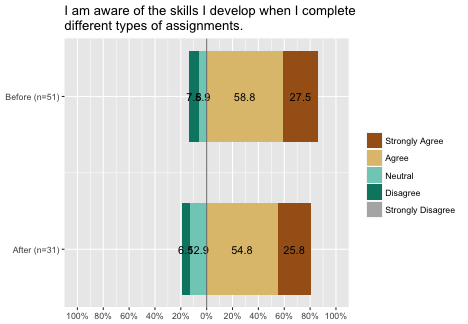
\includegraphics{figures/metacognition-3.png}

\begin{Shaded}
\begin{Highlighting}[]
\NormalTok{meta.data <-}\StringTok{ }
\StringTok{  }\NormalTok{merged.data %>%}
\StringTok{  }\NormalTok{dplyr::}\KeywordTok{select}\NormalTok{(}\KeywordTok{contains}\NormalTok{(}\StringTok{"What is your level of agreement on the following statements? [When a difficult assignment is given to me, I feel confident that I can complete it.]"}\NormalTok{)) %>%}
\StringTok{  }\KeywordTok{rename}\NormalTok{(}\StringTok{`}\DataTypeTok{Before}\StringTok{`} \NormalTok{=}\StringTok{ `}\DataTypeTok{What is your level of agreement on the following statements? [When a difficult assignment is given to me, I feel confident that I can complete it.]before}\StringTok{`}\NormalTok{,}
         \StringTok{`}\DataTypeTok{After}\StringTok{`} \NormalTok{=}\StringTok{  `}\DataTypeTok{What is your level of agreement on the following statements? [When a difficult assignment is given to me, I feel confident that I can complete it.]after}\StringTok{`}\NormalTok{) %>%}
\StringTok{  }\KeywordTok{mutate}\NormalTok{(}\StringTok{`}\DataTypeTok{Before}\StringTok{`}\NormalTok{=}\StringTok{ }\KeywordTok{factor}\NormalTok{(}\StringTok{`}\DataTypeTok{Before}\StringTok{`}\NormalTok{, }\DataTypeTok{levels=}\NormalTok{mylevels),}
         \StringTok{`}\DataTypeTok{After}\StringTok{`}\NormalTok{=}\StringTok{ }\KeywordTok{factor}\NormalTok{(}\StringTok{`}\DataTypeTok{After}\StringTok{`}\NormalTok{, }\DataTypeTok{levels=}\NormalTok{mylevels))}

\KeywordTok{sjp.likert}\NormalTok{(meta.data, }\DataTypeTok{title=}\StringTok{"When a difficult assignment is given to me, I feel confident that I can complete it"}\NormalTok{, }\DataTypeTok{cat.neutral=}\StringTok{'Neutral'}\NormalTok{)}
\end{Highlighting}
\end{Shaded}

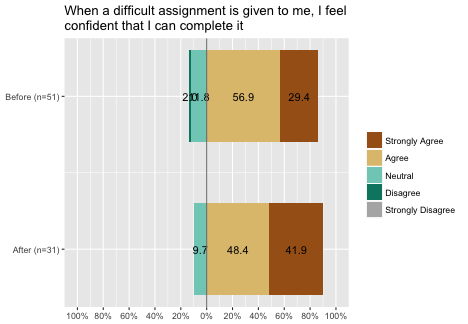
\includegraphics{figures/metacognition-4.png}

\begin{Shaded}
\begin{Highlighting}[]
\NormalTok{meta.data <-}\StringTok{ }
\StringTok{  }\NormalTok{merged.data %>%}
\StringTok{  }\NormalTok{dplyr::}\KeywordTok{select}\NormalTok{(}\KeywordTok{contains}\NormalTok{(}\StringTok{"What is your level of agreement on the following statements? [I perform better when completing an assignment that I enjoy (i.e., get a better grade).]"}\NormalTok{)) %>%}
\StringTok{  }\KeywordTok{rename}\NormalTok{(}\StringTok{`}\DataTypeTok{Before}\StringTok{`} \NormalTok{=}\StringTok{ `}\DataTypeTok{What is your level of agreement on the following statements? [I perform better when completing an assignment that I enjoy (i.e., get a better grade).]before}\StringTok{`}\NormalTok{,}
         \StringTok{`}\DataTypeTok{After}\StringTok{`} \NormalTok{=}\StringTok{  `}\DataTypeTok{What is your level of agreement on the following statements? [I perform better when completing an assignment that I enjoy (i.e., get a better grade).]after}\StringTok{`}\NormalTok{) %>%}
\StringTok{  }\KeywordTok{mutate}\NormalTok{(}\StringTok{`}\DataTypeTok{Before}\StringTok{`}\NormalTok{=}\StringTok{ }\KeywordTok{factor}\NormalTok{(}\StringTok{`}\DataTypeTok{Before}\StringTok{`}\NormalTok{, }\DataTypeTok{levels=}\NormalTok{mylevels),}
         \StringTok{`}\DataTypeTok{After}\StringTok{`}\NormalTok{=}\StringTok{ }\KeywordTok{factor}\NormalTok{(}\StringTok{`}\DataTypeTok{After}\StringTok{`}\NormalTok{, }\DataTypeTok{levels=}\NormalTok{mylevels))}

\KeywordTok{sjp.likert}\NormalTok{(meta.data, }\DataTypeTok{title=}\StringTok{"I perform better when completing an assignment that I enjoy (i.e., get a better grade)."}\NormalTok{, }\DataTypeTok{cat.neutral=}\StringTok{'Neutral'}\NormalTok{)}
\end{Highlighting}
\end{Shaded}

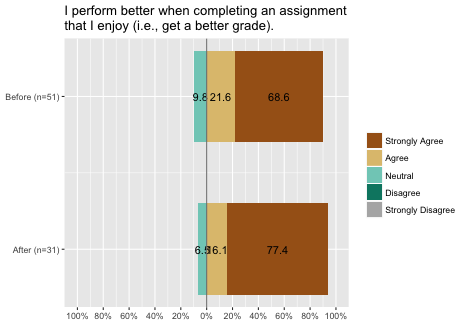
\includegraphics{figures/metacognition-5.png}

\section{Session Information}\label{session-information}

\begin{Shaded}
\begin{Highlighting}[]
\KeywordTok{sessionInfo}\NormalTok{()}
\end{Highlighting}
\end{Shaded}

\begin{verbatim}
## R version 3.4.2 (2017-09-28)
## Platform: x86_64-apple-darwin15.6.0 (64-bit)
## Running under: macOS High Sierra 10.13.3
## 
## Matrix products: default
## BLAS: /Library/Frameworks/R.framework/Versions/3.4/Resources/lib/libRblas.0.dylib
## LAPACK: /Library/Frameworks/R.framework/Versions/3.4/Resources/lib/libRlapack.dylib
## 
## locale:
## [1] en_US.UTF-8/en_US.UTF-8/en_US.UTF-8/C/en_US.UTF-8/en_US.UTF-8
## 
## attached base packages:
## [1] stats     graphics  grDevices utils     datasets  methods   base     
## 
## other attached packages:
## [1] sjPlot_2.4.0 bindrcpp_0.2 readr_1.1.1  dplyr_0.7.4  tidyr_0.7.2 
## [6] knitr_1.17  
## 
## loaded via a namespace (and not attached):
##  [1] nlme_3.1-131       RColorBrewer_1.1-2 rprojroot_1.2     
##  [4] tools_3.4.2        TMB_1.7.12         backports_1.1.1   
##  [7] R6_2.2.2           sjlabelled_1.0.6   DT_0.3            
## [10] lazyeval_0.2.1     colorspace_1.3-2   nnet_7.3-12       
## [13] tidyselect_0.2.3   mnormt_1.5-5       emmeans_1.1       
## [16] curl_3.0           compiler_3.4.2     cli_1.0.0         
## [19] sandwich_2.4-0     effects_4.0-0      scales_0.5.0      
## [22] lmtest_0.9-35      mvtnorm_1.0-7      psych_1.7.8       
## [25] blme_1.0-4         stringr_1.2.0      digest_0.6.12     
## [28] foreign_0.8-69     minqa_1.2.4        rmarkdown_1.8     
## [31] stringdist_0.9.4.6 pkgconfig_2.0.1    htmltools_0.3.6   
## [34] lme4_1.1-14        pwr_1.2-1          htmlwidgets_1.0   
## [37] rlang_0.1.4        rstudioapi_0.7     shiny_1.0.5       
## [40] bindr_0.1          zoo_1.8-1          magrittr_1.5      
## [43] modeltools_0.2-21  bayesplot_1.4.0    Matrix_1.2-12     
## [46] Rcpp_0.12.14       munsell_0.4.3      abind_1.4-5       
## [49] prediction_0.2.0   stringi_1.1.6      multcomp_1.4-8    
## [52] yaml_2.1.15        merTools_0.3.0     snakecase_0.8.1   
## [55] carData_3.0-0      MASS_7.3-47        plyr_1.8.4        
## [58] grid_3.4.2         parallel_3.4.2     sjmisc_2.6.3      
## [61] forcats_0.2.0      crayon_1.3.4       lattice_0.20-35   
## [64] ggeffects_0.3.1    haven_1.1.0        splines_3.4.2     
## [67] sjstats_0.14.0     hms_0.4.0          estimability_1.2  
## [70] reshape2_1.4.2     codetools_0.2-15   stats4_3.4.2      
## [73] glue_1.2.0         evaluate_0.10.1    modelr_0.1.1      
## [76] httpuv_1.3.5       nloptr_1.0.4       gtable_0.2.0      
## [79] purrr_0.2.4        assertthat_0.2.0   ggplot2_2.2.1     
## [82] mime_0.5           coin_1.2-2         xtable_1.8-2      
## [85] broom_0.4.3        survey_3.32-1      coda_0.19-1       
## [88] survival_2.41-3    tibble_1.3.4       arm_1.9-3         
## [91] glmmTMB_0.2.0      TH.data_1.0-8
\end{verbatim}


\end{document}
